\documentclass[tikz,border=10pt]{standalone}
\usetikzlibrary{positioning,calc}

\begin{document}
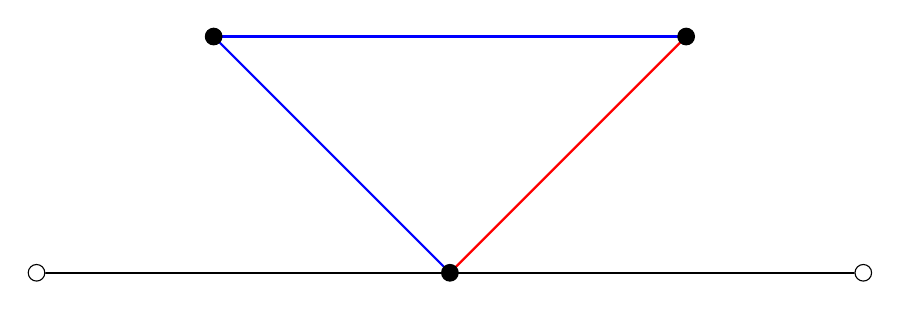
\begin{tikzpicture}[scale=1.5, transform shape]

% Coordinates for the vertices
\coordinate (A) at (-2,0);
\coordinate (B) at (2,0);
\coordinate (C) at (0,-2);

% Draw lines
\draw[thick, blue] (A) -- (B);
\draw[thick, blue] (A) -- (C);
\draw[thick, red] (B) -- (C);

% Horizontal line through point C
\draw[thick] ($(C) + (-3.5,0)$) -- ($(C) + (3.5,0)$);

% Mark points with circles
\filldraw[black] (A) circle (2pt);
\filldraw[black] (B) circle (2pt);
\filldraw[black] (C) circle (2pt);

% Open circles at ends of horizontal line
\filldraw[white] ($(C) + (-3.5,0)$) circle (2pt);
\filldraw[white] ($(C) + (3.5,0)$) circle (2pt);
\draw ($(C) + (-3.5,0)$) circle (2pt);
\draw ($(C) + (3.5,0)$) circle (2pt);

\end{tikzpicture}
\end{document}